\documentclass[sn-mathphys]{sn-jnl}

\AtBeginDocument{%
  \renewcommand\normalsize{\fontsize{8}{9}\selectfont}
  \renewcommand\small{\fontsize{8}{9}\selectfont}
  \renewcommand\footnotesize{\fontsize{6}{8}\selectfont}
}

\usepackage{comment}
\usepackage{graphicx}%
\graphicspath{{Images/}}
\usepackage{multirow}%
\usepackage{amsmath,amssymb,amsfonts}%
\usepackage{amsthm}%
\usepackage{mathrsfs}%
\usepackage[title]{appendix}%
%\usepackage{xcolor}%
\usepackage[table]{xcolor}
\usepackage{csquotes}
\usepackage[margin=1in]{geometry}
\usepackage{accents}
\usepackage{textcomp}%
\usepackage{manyfoot}%
\usepackage{booktabs}%
%\usepackage{algorithm}%
%\usepackage{algorithmicx}%
\usepackage{algpseudocode}%
\usepackage{listings}%
\usepackage{caption}
\usepackage{subcaption}
\usepackage{orcidlink}
\usepackage{hyperref}
\MakeOuterQuote{"}
\usepackage{etoolbox}
\usepackage{enumitem}
\usepackage{makecell}
\usepackage{url}
\usepackage[ruled,vlined,linesnumbered]{algorithm2e}

% Global settings for all enumerate environments:
\setlist[enumerate]{
  topsep=0pt,    % space above and below the list
  partopsep=0pt, % extra space when starting a new paragraph
  parsep=0.1em,    % space between paragraphs within an item
  itemsep=0.25em,
  font=\normalfont\normalsize}

% Global settings for all enumerate environments:
\setlist[itemize]{
  topsep=0pt,    % space above and below the list
  partopsep=0pt, % extra space when starting a new paragraph
  parsep=0.1em,    % space between paragraphs within an item
  itemsep=0.25em,
  font=\normalfont\normalsize}
  
%% as per the requirement new theorem styles can be included as shown below
\theoremstyle{thmstyleone}%
\newtheorem{theorem}{Theorem}%  meant for continuous numbers
%%\newtheorem{theorem}{Theorem}[section]% meant for sectionwise numbers
%% optional argument [theorem] produces theorem numbering sequence instead of independent numbers for Proposition
\newtheorem{proposition}[theorem]{Proposition}% 
%%\newtheorem{proposition}{Proposition}% to get separate numbers for theorem and proposition etc.
\setlength{\abovecaptionskip}{4pt}  % espace au-dessus de la légende
\setlength{\belowcaptionskip}{0pt}  % espace sous la légende
\theoremstyle{thmstyletwo}%
\newtheorem{example}{Example}%
\newtheorem{remark}{Remark}%

\theoremstyle{thmstylethree}%
\newtheorem{definition}{Definition}%

\raggedbottom
%%\unnumbered% uncomment this for unnumbered level heads

\let\oldthebibliography\thebibliography
\let\endoldthebibliography\endthebibliography
\renewenvironment{thebibliography}[1]{
  \begin{oldthebibliography}{#1}
    \setlength{\itemsep}{0em}
    \setlength{\parskip}{0em}
}
{
  \end{oldthebibliography}
}

\begin{document}

\title{Black-box Active Learning for Discovering New Explanations in Complex System Exploration}%

\author*[1]{\fnm{Paul} \sur{Saves}\orcidlink{0000-0001-5889-2302} }\email{paul.saves@irit.fr}
\author[1]{\fnm{Nicolas} \sur{Verstaevel}\orcidlink{0000-0002-7879-6681}  }\email{nicolas.verstaevel@irit.fr}
\author[1]{\fnm{Benoit} \sur{Gaudou}\orcidlink{0000-0002-9005-3004 }}\email{benoit.gaudou@ut-capitole.fr}
\affil*[1]{\orgdiv{Université Toulouse Capitole, IRIT},  \city{Toulouse}, \postcode{31000},\state{Occitanie},\country{ France}}

\abstract{
Exploring the parameter space of complex socio-technical systems, such as Agent-Based Models (ABMs), presents significant challenges due to inherent high dimensionality and computational cost. As these simulators typically function as non-differentiable black boxes, effective exploration requires derivative-free strategies. However, traditional sampling methods, such as Stepwise Uncertainty Reduction (SUR) or static Designs of Experiments (DoE), typically prioritize minimizing global prediction error or output variance. These approaches often fail to capture the diverse causal mechanisms underlying system behavior, thereby missing critical behavioral regimes where different input combinations yield similar macroscopic outputs for fundamentally different reasons.

In this work, we propose a novel black-box active learning framework designed to discover novel explanatory structures rather than simply accumulating data points. Our model-agnostic method integrates surrogate modeling with post-hoc Explainable Artificial Intelligence (XAI) to guide the exploration process. The methodology proceeds in an iterative Bayesian loop, maximizing the explanatory diversity within the collected data. By explicitly targeting points that are distinct in their explanatory structure—i.e., their feature contribution profiles—our framework efficiently uncovers rare behavioral regimes and distinct internal logic.
Consequently, this framework achieves a deeper structural understanding with fewer simulations than standard prediction-based strategies. It proves particularly effective in characterizing critical system behaviors, including tipping points. 

\textbf{Keywords:} Surrogate models $\cdot$  Explainable Artificial Intelligence $\cdot$ Machine learning  $\cdot$ Active Learning  $\cdot$ Agent-based modeling 
}

\maketitle

\tableofcontents

\section{Introduction}
Simulations of complex socio-technical systems, such as Agent-Based Models (ABMs), are vital for understanding emergent phenomena. However, the exploration of their parameter spaces is often bottlenecked by computational costs and inherent high dimensionality. These simulators generally act as non-differentiable black boxes, rendering traditional gradient-based optimization ineffective. 

In dynamical systems, tipping points are classically viewed as mathematical discontinuities or bifurcations where the derivative of the state variables approaches infinity (Scheffer et al., 2009). Proving such analytical discontinuities is impossible from finite samples in stochastic, derivative-free ABMs. Therefore, we mathematically relax this constraint: instead of seeking an infinite gradient, we define a generalized tipping point as a localized region exhibiting a locally bounded but extremely large Lipschitz constant. Because ABMs are stochastic (where the response $Y(x) = \mu(x) + \varepsilon(x)$), we frame this via probabilistic bounds on the expected response: $\mathbb{P}(\nabla \mu(x) > \tau) > 1 - \delta$. By systematically targeting these regions where the model's causal logic undergoes substantial shifts, we can locate these out-of-equilibrium phase transitions without solving differential equations. To properly track these non-smooth transitions, the underlying surrogate model requires a rougher covariance structure, making a Matérn $3/2$ or $1/2$ kernel strictly preferable to infinitely differentiable squared-exponential (RBF) kernels.

To reduce the computational burden of sampling-intensive tasks, researchers traditionally employ surrogate models (e.g., Kriging/Gaussian Processes) coupled with sampling strategies like static DoE or adaptive sampling via Bayesian Optimization. While these methods excel at minimizing global prediction error or finding global optima, they fall short in uncovering the diverse causal mechanisms that drive system behavior. They frequently miss complex behavioral regimes where different parameter combinations yield similar macroscopic outputs for fundamentally different internal reasons.

To address this, we introduce a model-agnostic active learning framework that couples surrogate modeling with Explainable Artificial Intelligence (XAI). Rather than targeting prediction uncertainty, our approach actively queries for novel explanatory profiles. By utilizing tools such as SHAP (SHapley Additive exPlanations) to interpret feature contributions, our methodology iteratively samples points that exhibit rare or unseen explanatory profiles, efficiently mapping the boundaries of complex system behaviors and tipping points.

\section{Methods}
To operationalize the search for novel explanations introduced above, we developed a five-step framework. Our proposed methodology relies on an iterative Bayesian active learning loop designed to maximize explanatory diversity[cite: 19]. The workflow consists of five primary steps:

\begin{enumerate}
    \item \textbf{Pre-Processing: Handling ABM Stochasticity:} Agent-Based Models are inherently stochastic. To construct a reliable deterministic surrogate model (Kriging), we must "remove" this aleatoric noise by estimating the true mean response. We dynamically execute replications until the variance of the mean stabilizes, verified online using an F-test (Fisher test) to ensure sufficient statistical power and minimize Type-II false negatives (Secchi \& Seri, 2017; Lorscheid et al., 2012).
    
    \item \textbf{Initial Dataset Generation (The LHS-ESE Baseline):} We compare our approach against the gold-standard static DoE: Latin Hypercube Sampling optimized via Enhanced Stochastic Evolutionary (LHS-ESE). Formulated as a constrained optimization problem, it globally minimizes the Minkowski norm ($L_p$) of the inverse of the Euclidean distances in the search space ($\Phi_p$ criterion by Morris \& Mitchell) using the discrete combinatorial ESE algorithm (Jin et al., 2005). We generate an initial set of $n_{doe}$ points within the feature design space and evaluate them using the simulator to obtain the deterministic outputs $y_{doe}$.
    
    \item \textbf{Explanation Inputs and Constructing the Dual Space:} We map the physical space to a causal explanatory space using cooperative game theory. For any feature coalition $S \subseteq F$, the SHAP value function is defined as the conditional expectation $v(S) = \mathbb{E}[f(X) \mid X_S = x_S]$. The exact combinatorial feature contributions are computed as $\phi_i(x) = \sum_{S \subseteq F \setminus \{i\}} \frac{|S|! (|F| - |S| - 1)!}{|F|!} (v(S \cup \{i\}) - v(S))$. These SHAP values distribute the exact difference between the local prediction and the global average: $\sum \phi_i(x) = f(x) - \mathbb{E}[f(X)]$, mapping each physical point $x$ to its local explanatory profile $S(x)$. To bypass the cost of generating explanations directly from the simulator, we train a noisy Gaussian Process (GP) on the initial dataset $\{x_{doe}, y_{doe}\}$. We then sample $n_{xpl\_lowfi}$ low-fidelity points ($x_{xpl\_lowfi}$) in the design space. Using the GP as a proxy, we compute ExactSHAP values for both the evaluated points and the low-fidelity points. Crucially, we use the initial stationary LHS sample as the fixed background reference to ensure the explanatory space remains historically comparable across active learning iterations. 
    
    \item \textbf{Explanation Novelty via Fast Proxy:} To bypass the curse of dimensionality inherent in high-dimensional KDE, where $L_2$ distances suffer from the concentration of measure, we quantify the novelty of an explanation using a Fast Density Proxy via Cosine Distance (Nearest Neighbors) on the generated SHAP values. By focusing on the directional alignment of feature contributions, the proxy preserves the local manifold structure. We define the density proxy as the average cosine distance over the $k$ nearest neighbors:
    \begin{equation}
        \rho_{proxy}(x) \propto \exp\left( -\gamma \cdot \frac{1}{k} \sum_{j=1}^k \left(1 - \frac{S(x) \cdot S_{(j)}}{||S(x)|| \, ||S_{(j)}||}\right) \right)
    \end{equation}
    This yields a novelty metric $y_{nov\_total}$[cite: 61]. The dataset is split into high-fidelity novelties ($y_{nov\_high}$ corresponding to $x_{doe}$) and low-fidelity novelties ($y_{nov\_low}$ corresponding to $x_{xpl\_lowfi}$)[cite: 62]. Areas with high cosine distance indicate rare or novel explanatory structures.
    
    \item \textbf{Dynamic Hybrid Bayesian Optimization (Dynamic-US):} We construct a Multi-Fidelity Gaussian Process (MFGP) using the combined datasets: $[\{x_{doe}, y_{nov\_high}\}, \{x_{xpl\_lowfi}, y_{nov\_low}\}]$[cite: 80]. Rather than purely optimizing explanatory novelty, we frame the acquisition strategy as a bi-objective optimization problem. The goal is to simultaneously \textbf{minimize} physical uncertainty (the Integrated Mean Squared Error $\text{IMSE}_{MC}(x)$) and \textbf{maximize} explanatory exploitation (the novelty derived from cosine distance to the historical SHAP dataset, represented by $\text{EI}_{MFK}(x)$). We formalize physical exploration as a Stepwise Uncertainty Reduction (SUR) strategy: $\Delta\text{IMSE}(x) = \int_{\mathcal{X}} \left( \sigma^2_n(x') - \sigma^2_{n+1}(x' \mid x) \right) \text{d}x'$, approximated via a discrete Monte-Carlo grid ($N_{MC} \in [100, 500]$) following the Kriging Believer heuristic (where the surrogate is temporarily updated with its own mean prediction at the candidate point). Because we actively maximize the acquisition function, we scalarize the problem utilizing dynamic min-max normalization to prevent magnitude domination and outlier collapse:
    \begin{equation}
        a_{Dynamic}(x) = (1 - \alpha^{(t)}) \cdot \frac{\Delta\text{IMSE}_{MC}(x) - \min}{\max - \min} + \alpha^{(t)} \cdot \frac{\widetilde{\text{EI}}_{MFK}(x) - \min}{\max - \min}
    \end{equation}
    The parameter $\alpha^{(t)}$ smoothly sweeps the Pareto front across iterations via a dynamic schedule $\alpha^{(t)} = \alpha_{start} + (\alpha_{end} - \alpha_{start}) \frac{t}{T}$. To ensure robust asymptotic convergence, we bound the exploration-exploitation trade-off using $\alpha_{start} = 0.01$ and $\alpha_{end} = 0.90$. This highly multimodal acquisition surface is optimized locally yet aggressively using a Derivative-Free Mixed-Integer Differential Evolution algorithm. To ensure computational tractability against the expensive IMSE grid evaluation, the Differential Evolution is initialized directly from a 50-point LHS population and strictly bounded to a maximum of 5 iterations[cite: 81]. Ultimately, by balancing physical uncertainty with explanatory novelty, the algorithm is forced to sample the exact parameter boundaries where the model's internal logic shifts, successfully isolating the tipping points.
    
    \item \textbf{Update:} The expensive black-box simulator is queried at the new point $x_{opt}$ to retrieve $y_{opt}$[cite: 102]. The exact dataset is then updated ($x_{doe} := x_{doe} \cup x_{opt}$ and $y_{doe} := y_{doe} \cup y_{opt}$), and the loop repeats[cite: 103, 104].
\end{enumerate}

\subsection{Connection to Active Subspaces}
The proposed methodology inherently performs a dynamic dimensionality reduction. Active Subspace methods find a covariance matrix $C = \int (\nabla f(x))(\nabla f(x))^T \rho(x) dx$. Under infinitesimal perturbations, the SHAP value is approximately $\phi_i(x) \approx \frac{\partial f(x)}{\partial x_i} (x_i - \mathbb{E}[X_i])$. Therefore, the outer product of the SHAP vectors is proportional to the gradient outer product, weighted by the variance of the input space: $S(x)S(x)^T \approx (\nabla f(x) \odot (x - \mathbb{E}[x])) (\nabla f(x) \odot (x - \mathbb{E}[x]))^T$. Assuming the input space is standardized, the covariance matrix of the SHAP values formally approximates the Active Subspace matrix $C$. By performing Cosine KNN on $S(x)$, the algorithm clusters points based on their directional alignment within this Active Subspace. Thus, explicitly hunting for SHAP novelty is mathematically equivalent to tracking the rotation of the Active Subspace, which proves highly effective at mapping complex, non-linear tipping points. Furthermore, because the surrogate model $f(x)$ is a Gaussian Process ($f \sim \mathcal{GP}(\mu, K)$), any linear operator applied to it—such as the SHAP value integration—results in another Gaussian Process. Thus, the SHAP values themselves are random variables with a computable posterior distribution $\mathcal{N}(\mu_{SHAP}(x), \Sigma_{SHAP}(x))$, enabling future theoretical extensions to measure "Explanatory Uncertainty".

\begin{algorithm}[hbt!]
\SetAlgoLined
\KwIn{Expensive black-box simulator $f$, Feature design space $\mathcal{X}$, Initial budget $n_{doe}$, Total budget $N$, Low-fidelity explanation budget $n_{xpl\_lowfi}$}
\KwOut{Explored dataset $\mathcal{D} = \{x_{doe}, y_{doe}\}$}

\vspace{2mm}
\tcp{Step 1: Initial Dataset Generation}
Optimize an initial Latin Hypercube Sample (LHS-ESE) of size $n_{doe}$ by minimizing the Minkowski distance $\Phi_p$\;
Execute an initial $n_{min}$ replications per point. \textbf{While} sequential stopping rule condition $\frac{S_n(x)}{\sqrt{n}} t_{\alpha/2, n-1} > \delta$ holds, increment $n$ and simulate to estimate the true mean response: $\hat{y}_{doe} \leftarrow \mathbb{E}[f(x_{doe})]$\;
Initialize dataset $\mathcal{D} \leftarrow \{x_{doe}, \hat{y}_{doe}\}$\;
Initialize dynamic scalarization weight: $\alpha^{(0)} \leftarrow \alpha_{start}$\;
Define step size $\Delta \alpha = \frac{\alpha_{end} - \alpha_{start}}{N - n_{doe} - 1}$\;
Initialize iteration counter $t \leftarrow 0$\;

\vspace{2mm}
\tcp{Active Learning Loop}
\While{$|\mathcal{D}| < N$}{
    \vspace{1mm}
    \tcp{Step 2: Explanation Inputs and Surrogate Training}
    Train a noisy Gaussian Process (GP) on the current dataset $\mathcal{D}$\;
    Sample $n_{xpl\_lowfi}$ points $x_{xpl\_lowfi}$ in $\mathcal{X}$\;
    \textbf{If} dimension $M > 15$, utilize KernelSHAP approximation to constrain complexity; \textbf{Else}, compute ExactSHAP values $S$ for $(x_{xpl\_lowfi} \cup x_{doe})$ using the GP as a proxy, with the stationary initial LHS as the background reference\;
    
    \vspace{2mm}
    \tcp{Step 3: Explanation Novelty}
    Compute proxy novelty $y_{nov\_total}$ on the SHAP values $S$ using Cosine Distance (k-NN)\;
    Extract high-fidelity novelties: $y_{nov\_high} \leftarrow y_{nov\_total}(x_{doe})$\;
    Extract low-fidelity novelties: $y_{nov\_low} \leftarrow y_{nov\_total}(x_{xpl\_lowfi})$\;

    Train a Multi-Fidelity Gaussian Process (MFGP) to predict explanation density using high-fidelity data $\{x_{doe}, y_{nov\_high}\}$ and low-fidelity data $\{x_{xpl\_lowfi}, y_{nov\_low}\}$\;

    \vspace{2mm}
    \tcp{Step 4: Dynamic Hybrid Bayesian Optimization}
    Generate an LHS initial population $\mathcal{P}_{init}$ of size 50 to ensure optimal spatial coverage\;
    Solve the optimization problem using a global Derivative-Free Mixed-Integer Differential Evolution initialized with $\mathcal{P}_{init}$\;
    To prevent magnitude domination, objectives are dynamically normalized relative to their minimums and maximums observed in the current Differential Evolution generation:\;
    $x_{opt} = \arg\max_{x \in \mathcal{X}} \left[ (1 - \alpha^{(t)}) \cdot \frac{\Delta\text{IMSE}_{MC}(x) - \min}{\max - \min} + \alpha^{(t)} \cdot \frac{\widetilde{\text{EI}}_{MFK}(x) - \min}{\max - \min} \right]$\;
    
    \vspace{2mm}
    \tcp{Step 5: Update}
    Execute an initial $n_{min}$ replications at the new point $x_{opt}$. \textbf{While} $\frac{S_n(x_{opt})}{\sqrt{n}} t_{\alpha/2, n-1} > \delta$, increment $n$ and simulate to estimate the mean response: $\hat{y}_{opt} \leftarrow \mathbb{E}[f(x_{opt})]$\;
    Update inputs: $x_{doe} \leftarrow x_{doe} \cup \{x_{opt}\}$\;
    Update outputs: $\hat{y}_{doe} \leftarrow \hat{y}_{doe} \cup \{\hat{y}_{opt}\}$\;
    Update dataset: $\mathcal{D} \leftarrow \{x_{doe}, \hat{y}_{doe}\}$\;
    Update scalarization weight: $\alpha^{(t+1)} \leftarrow \alpha^{(t)} + \Delta \alpha$\;
    $t \leftarrow t + 1$\;
}
\caption{Black-box Active Learning for Discovering New Explanations}
\label{algo:active_learning}
\end{algorithm}




\subsection{Identification of Rare Explanatory Regimes}

To evaluate the framework's ability to uncover distinct internal logic, we analyze the distribution of feature contributions using SHAP summary plots (see Figure X). Traditional space-filling designs often over-sample the homogenous regions of the parameter space, resulting in a dense clustering of SHAP values near zero, where features exert minimal distinct influence on the macroscopic output.

Conversely, our active learning loop, driven by the Cosine Distance Density Proxy on SHAP values, explicitly populates the sparse "tails" and isolated clusters of the distribution. By securing physical boundaries before pivoting to explanatory novelty, Dynamic-US identifies the true underlying transition boundaries better than pure SHAP novelty search, which often gets trapped in inaccurate surrogate spaces. For example, the SHAP beeswarm plot reveals distinct behavioral regimes where minor parameter adjustments dominate the model's convergence state. 

These low-density, high-impact regions represent critical tipping points in the Agent-Based Model, identified by systematically targeting exceptionally high Lipschitz constants (extreme finite-difference variations) in the explanatory manifold. By treating the SHAP density as a low-fidelity information source in the Multi-Fidelity Gaussian Process (MFGP), the optimization successfully targets these boundaries. The resulting dataset achieves a higher explanatory diversity, ensuring that the surrogate model not only predicts the output accurately but captures the diverse causal mechanisms that drive those predictions.
\section{Results}
Having established the theoretical mechanism of the Dynamic-US framework, we now evaluate its ability to empirically isolate tipping points. To validate the framework, testing was conducted on two robust Agent-Based Models: the Schelling segregation model and the MASTIO industrial symbiosis model. For both models, we compare the baseline LHS-ESE strategy against pure physical uncertainty reduction (IMSE-US), pure explanatory novelty (SHAP-US), and our proposed hybrid approach (Dynamic-US).

\subsection{Targeting Tipping Points in Parameter Space}
Traditional space-filling designs suffer from the curse of dimensionality, spreading samples uniformly and missing critical transition boundaries.
\begin{figure}[hbt!]
    \centering
    \begin{subfigure}{0.49\textwidth}
        
\includegraphics[width=\textwidth]{Images/Schelling/hybrid_diff_profile.png}
        \caption{Schelling}
    \end{subfigure}
    \begin{subfigure}{0.49\textwidth}
        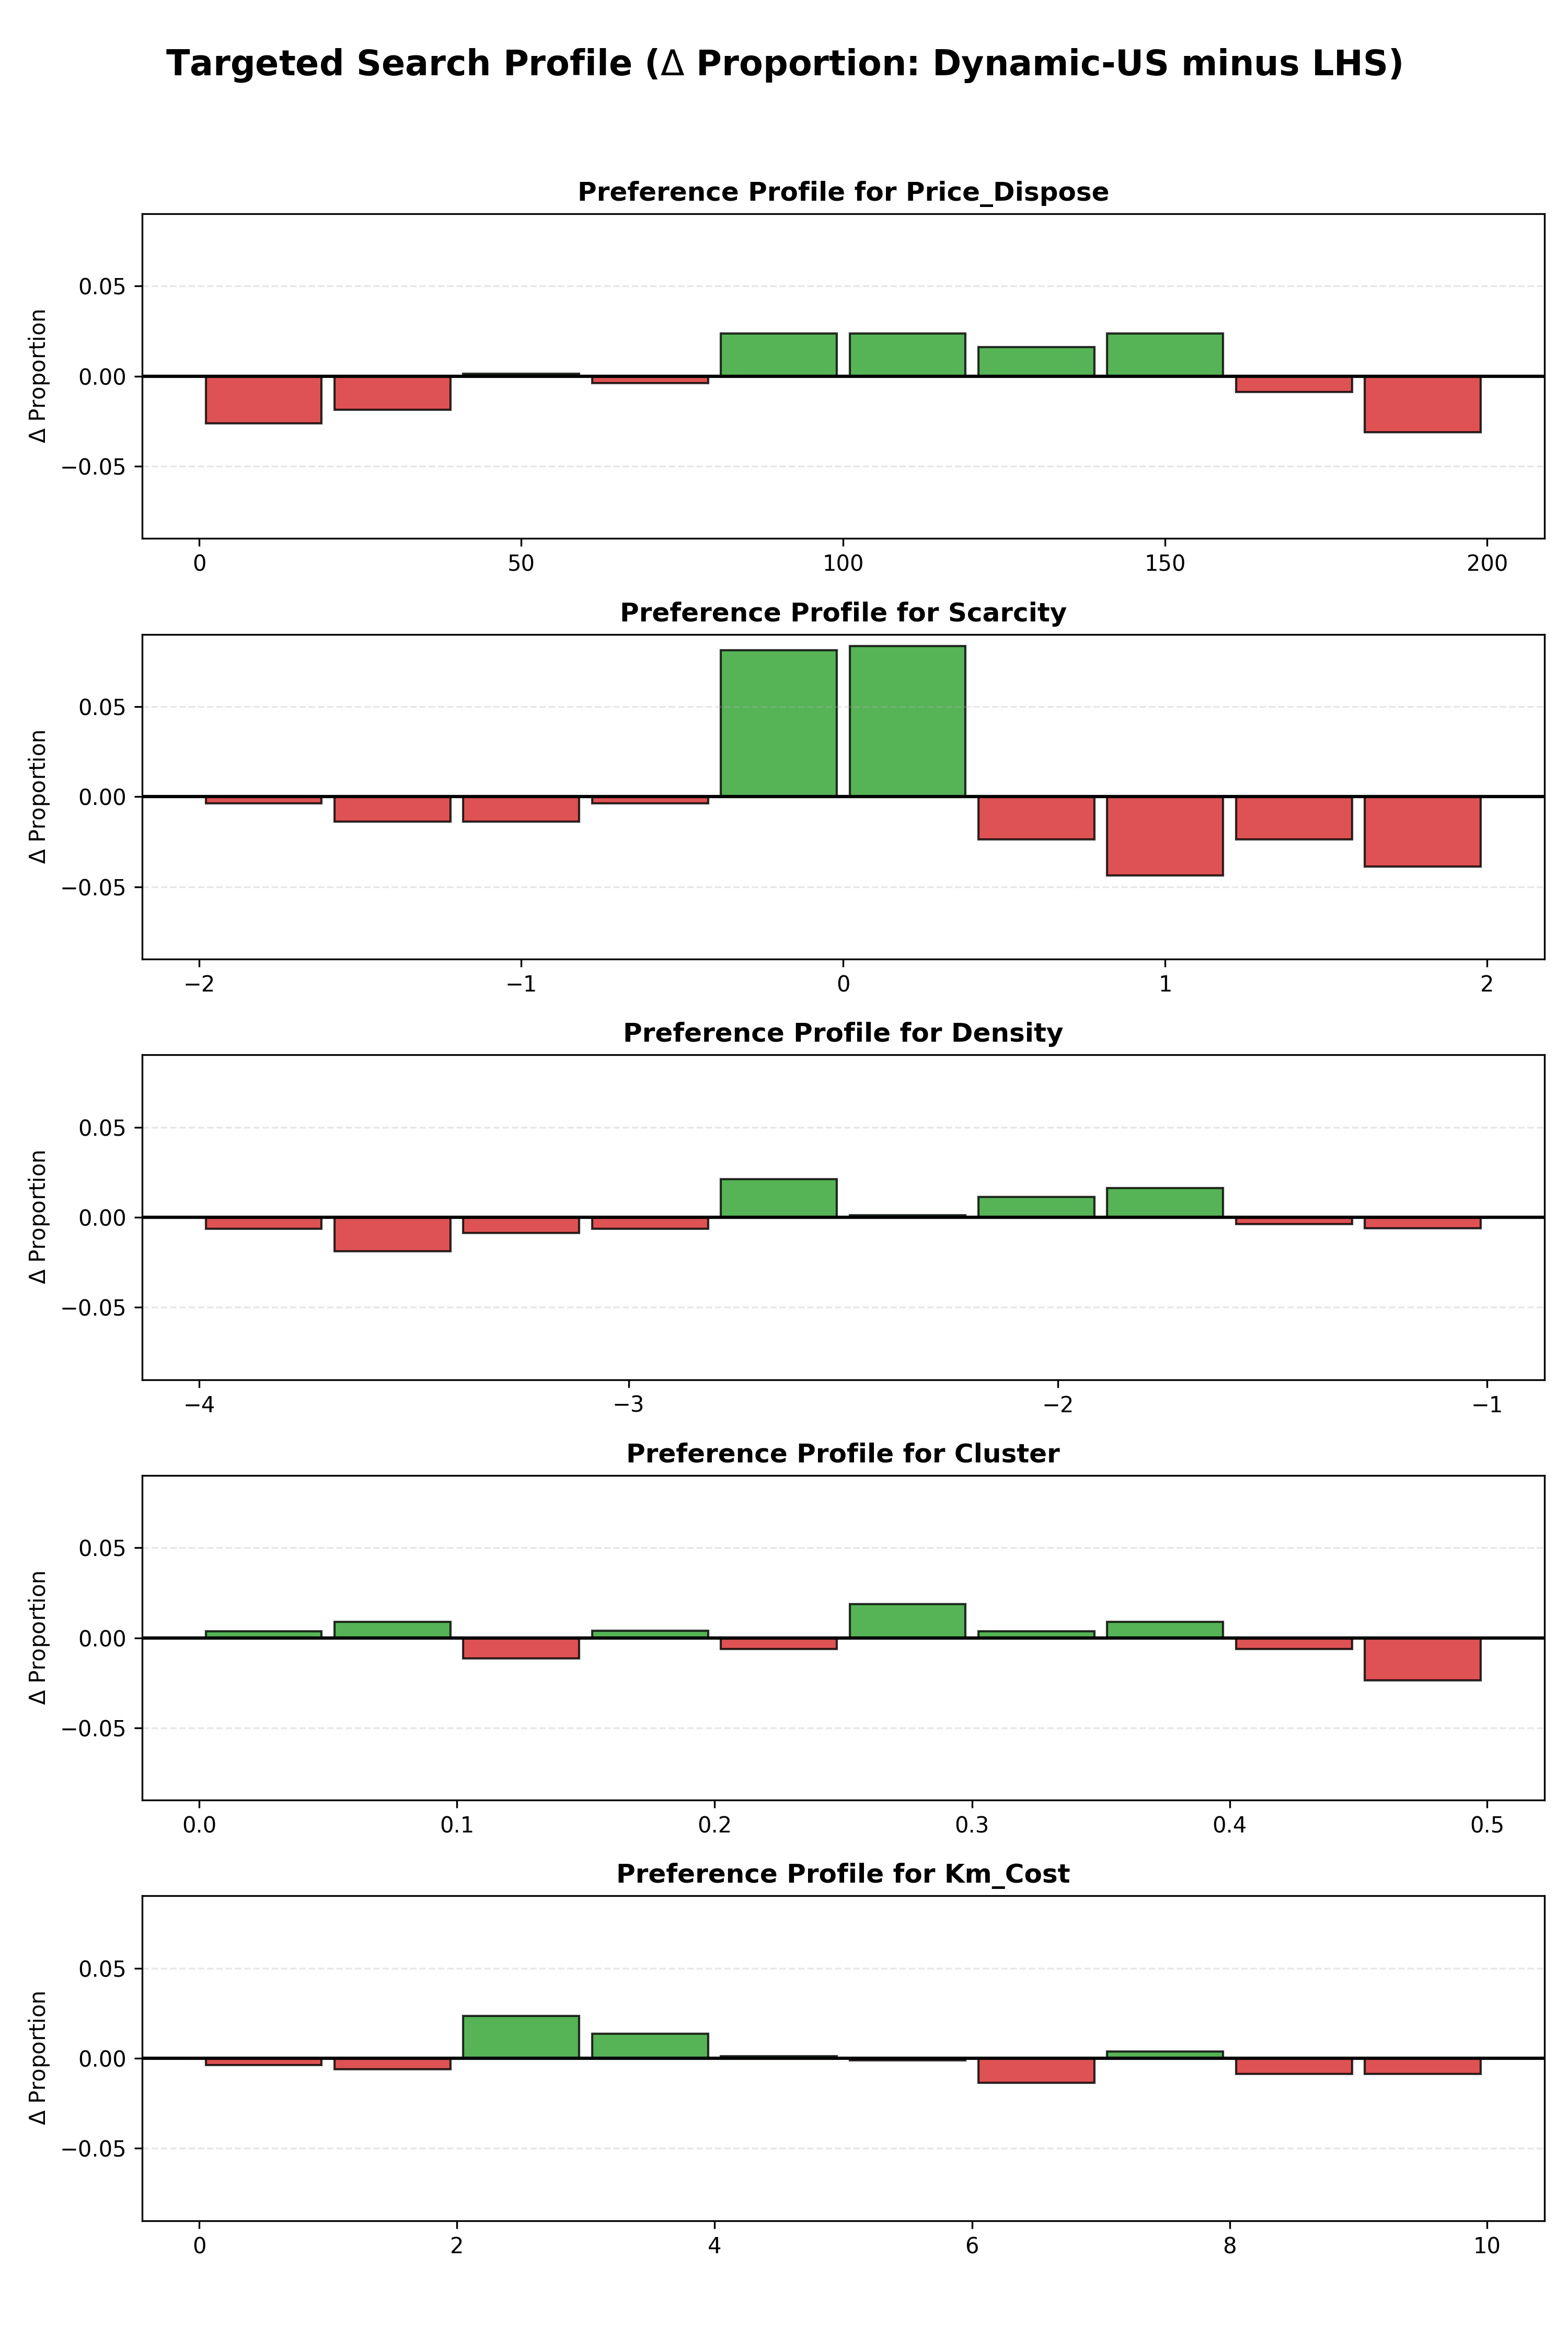
\includegraphics[width=\textwidth]{Images/MASTIO/hybrid_diff_profile.png}
        \caption{MASTIO}
    \end{subfigure}
    \caption{Hybrid density difference profile (\textbf{Dynamic-US minus LHS}). Green regions indicate narrow parameter bands intentionally over-sampled by the active learner, while red regions are actively ignored.}
    \label{fig:hybrid_diff}
\end{figure}

As shown by the 1D parameter histograms, the algorithm dynamically identifies and over-samples the specific parameter thresholds where the system's logic fundamentally changes.
\begin{figure}[hbt!]
    \centering
    \begin{subfigure}{0.49\textwidth}
        
\includegraphics[width=\textwidth]{Images/Schelling/1d_histograms_variables.png}
        \caption{Schelling 1D Histograms}
    \end{subfigure}
    \begin{subfigure}{0.49\textwidth}
        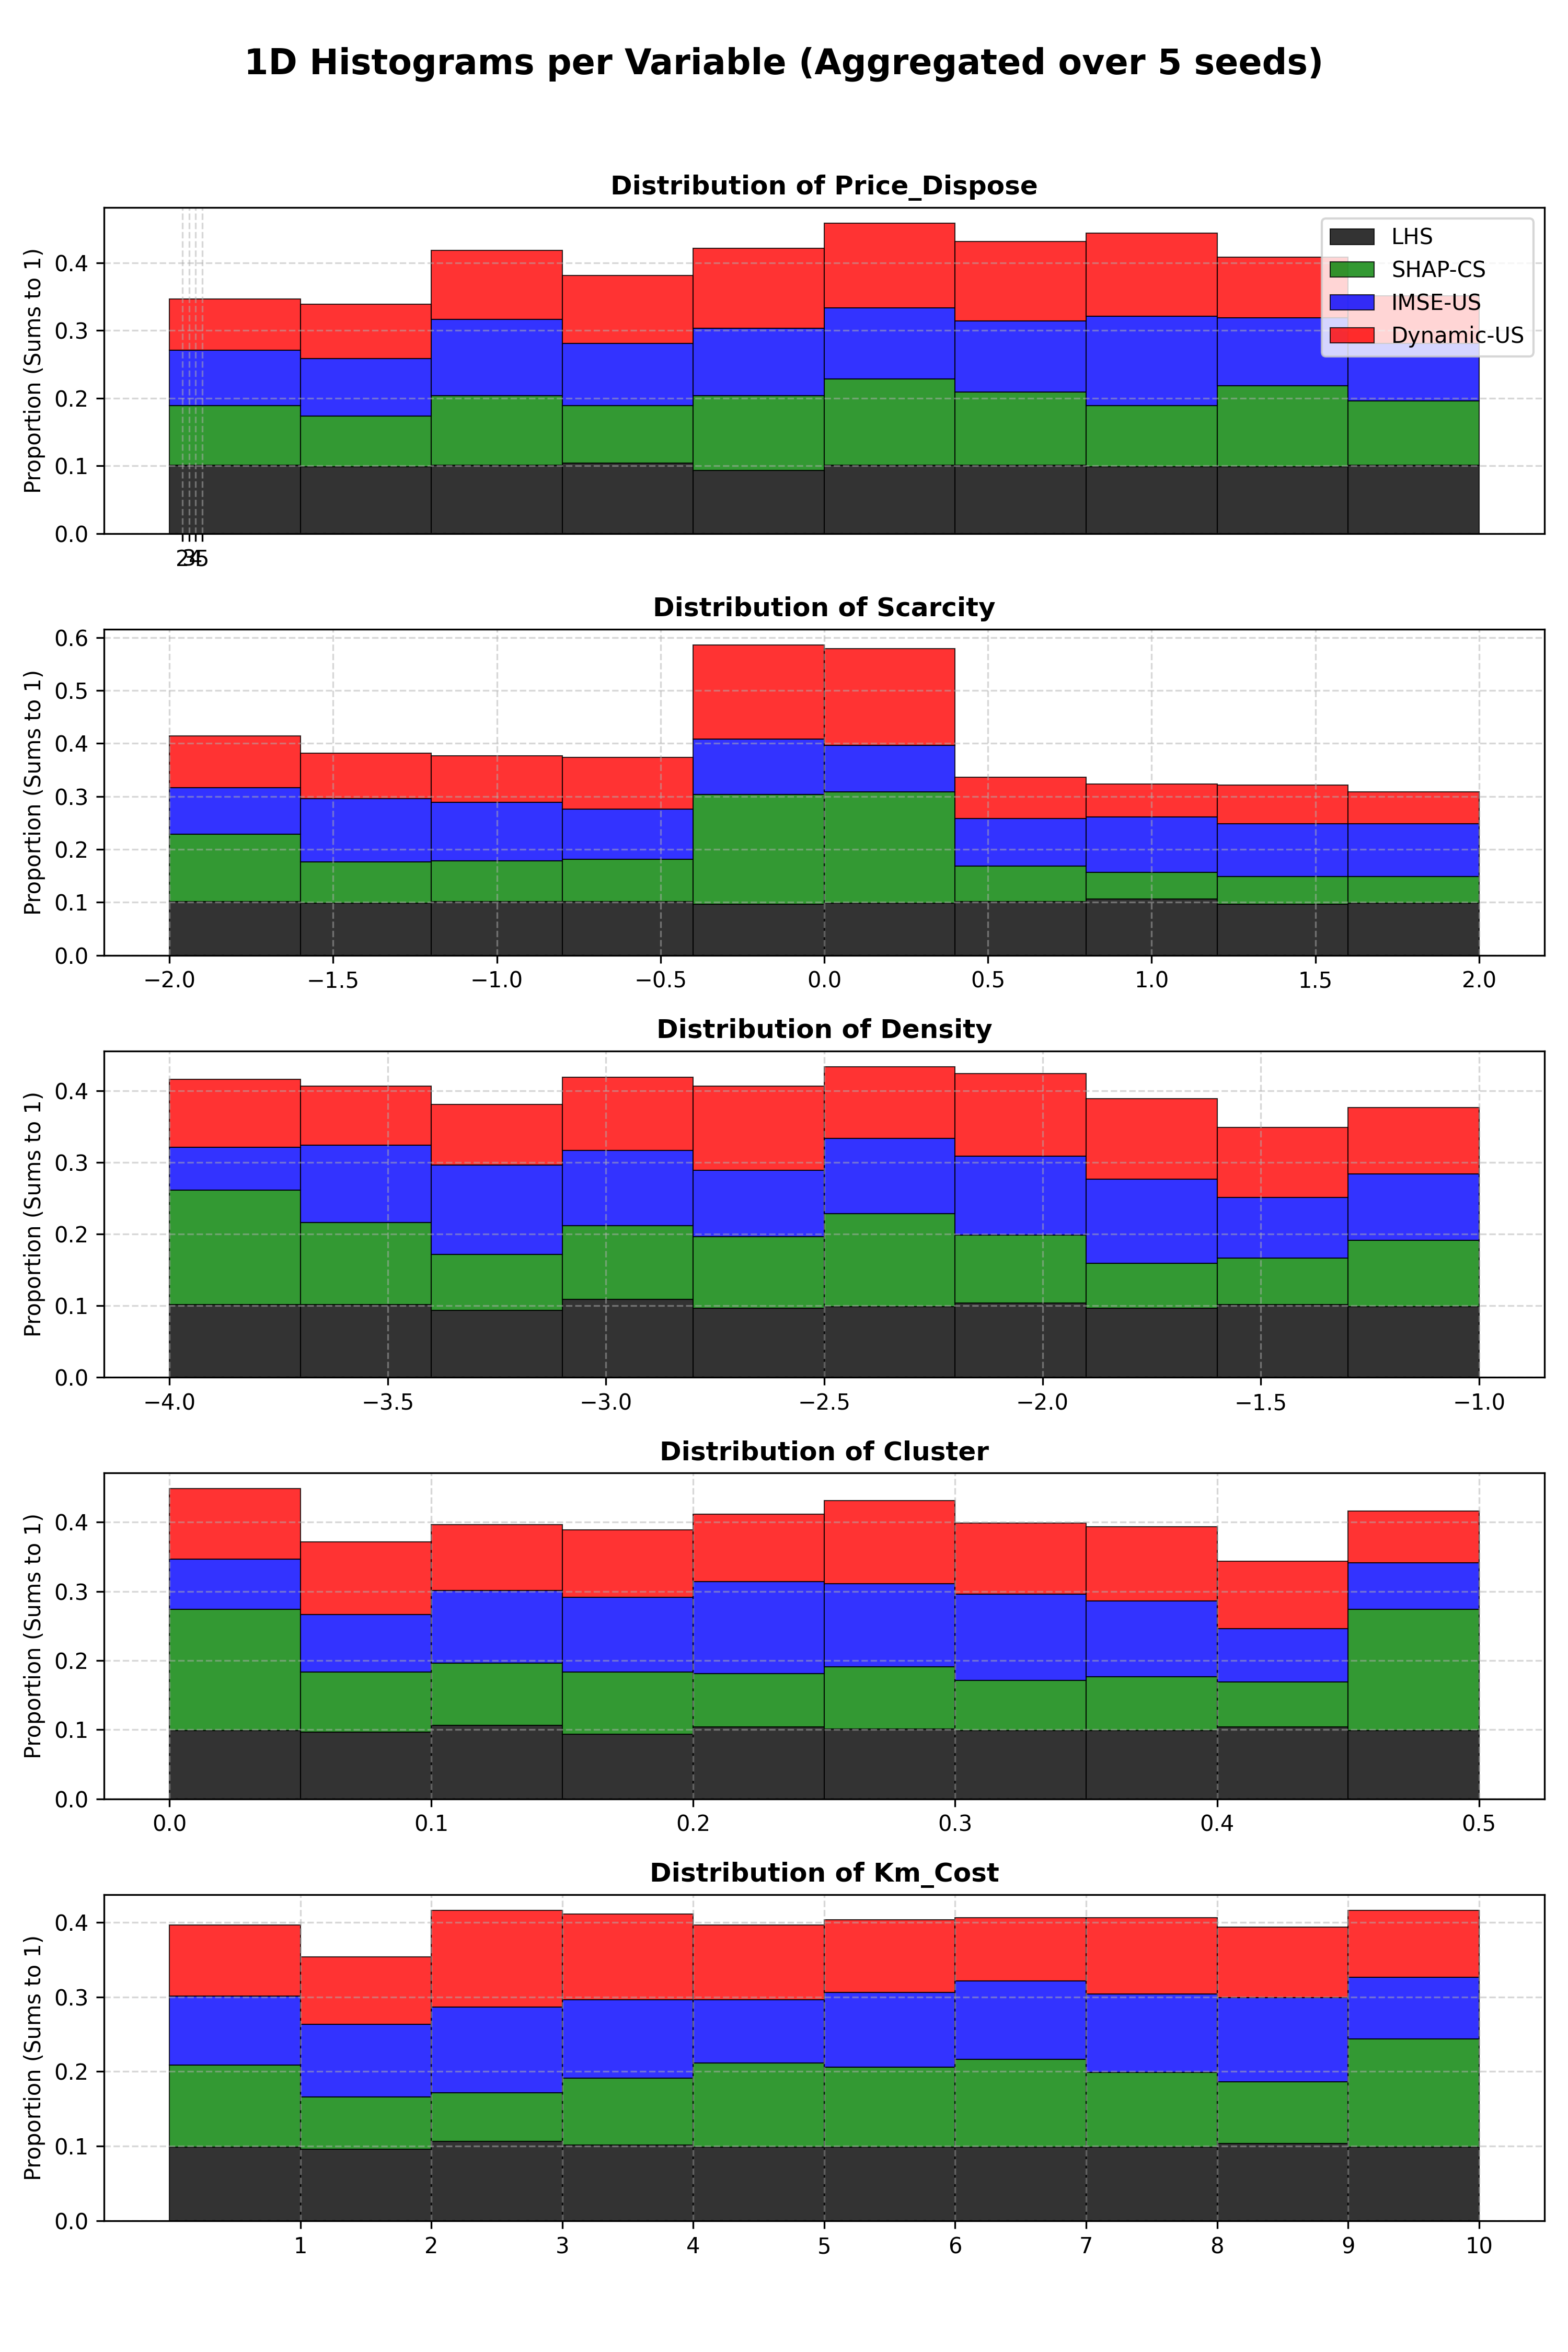
\includegraphics[width=\textwidth]{Images/MASTIO/1d_histograms_variables.png}
        \caption{MASTIO 1D Histograms}
    \end{subfigure}
    \caption{Parameter space sampling distribution. The hybrid method explicitly targets specific parameter thresholds corresponding to tipping points rather than uniformly mapping the space.}
    \label{fig:1d_histograms}
\end{figure}

\subsection{Tracking Tipping Points in Explanatory Space}
To visualize the exploration in the causal domain, we project the high-dimensional SHAP values into a 2D space using Principal Component Analysis (PCA). 
\begin{figure}[hbt!]
    \centering
    \begin{subfigure}{0.49\textwidth}
        
\includegraphics[width=\textwidth]{Images/Schelling/tipping_points_pca.png}
        \caption{Schelling PCA Evolution}
    \end{subfigure}
    \begin{subfigure}{0.49\textwidth}
        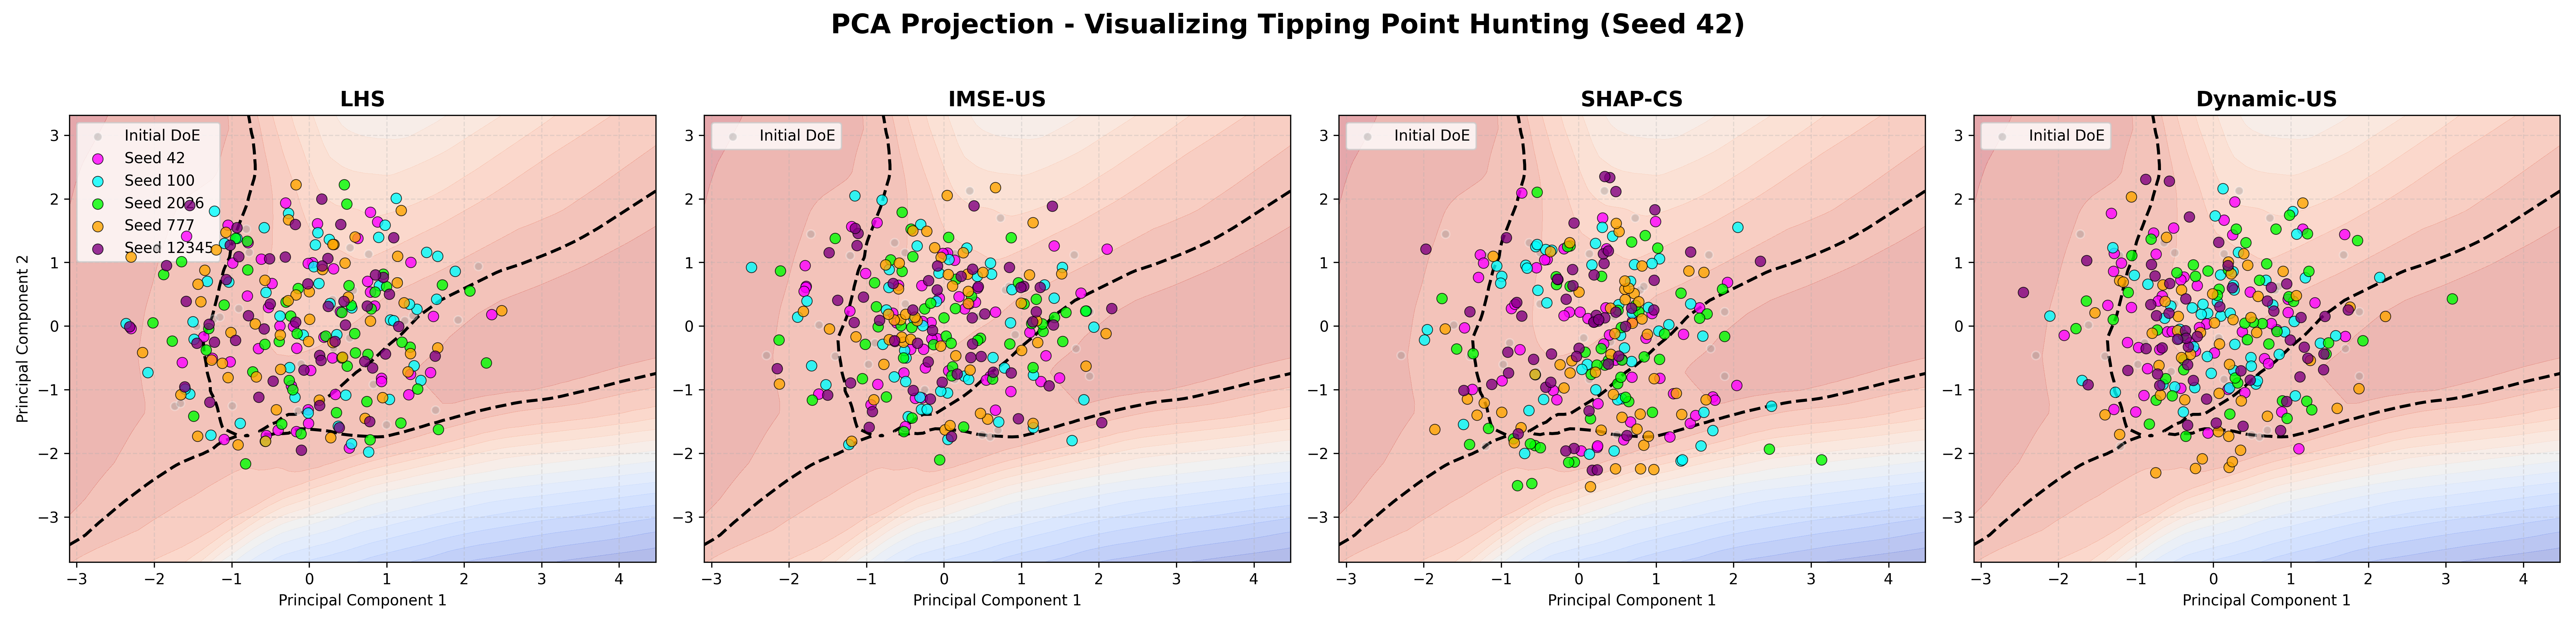
\includegraphics[width=\textwidth]{Images/MASTIO/tipping_points_pca.png}
        \caption{MASTIO PCA Evolution}
    \end{subfigure}
    \caption{PCA projection of the SHAP explanatory space for all methods. Dynamic-US efficiently tracks the non-linear boundaries where physical tipping points reside by actively querying for explanatory novelty.}
    \label{fig:pca_all}
\end{figure}

\begin{figure}[hbt!]
    \centering
    \begin{subfigure}{0.49\textwidth}
        
\includegraphics[width=\textwidth]{Images/Schelling/tipping_points_pca_final_shap.png}
        \caption{Schelling Final SHAP Space}
    \end{subfigure}
    \begin{subfigure}{0.49\textwidth}
        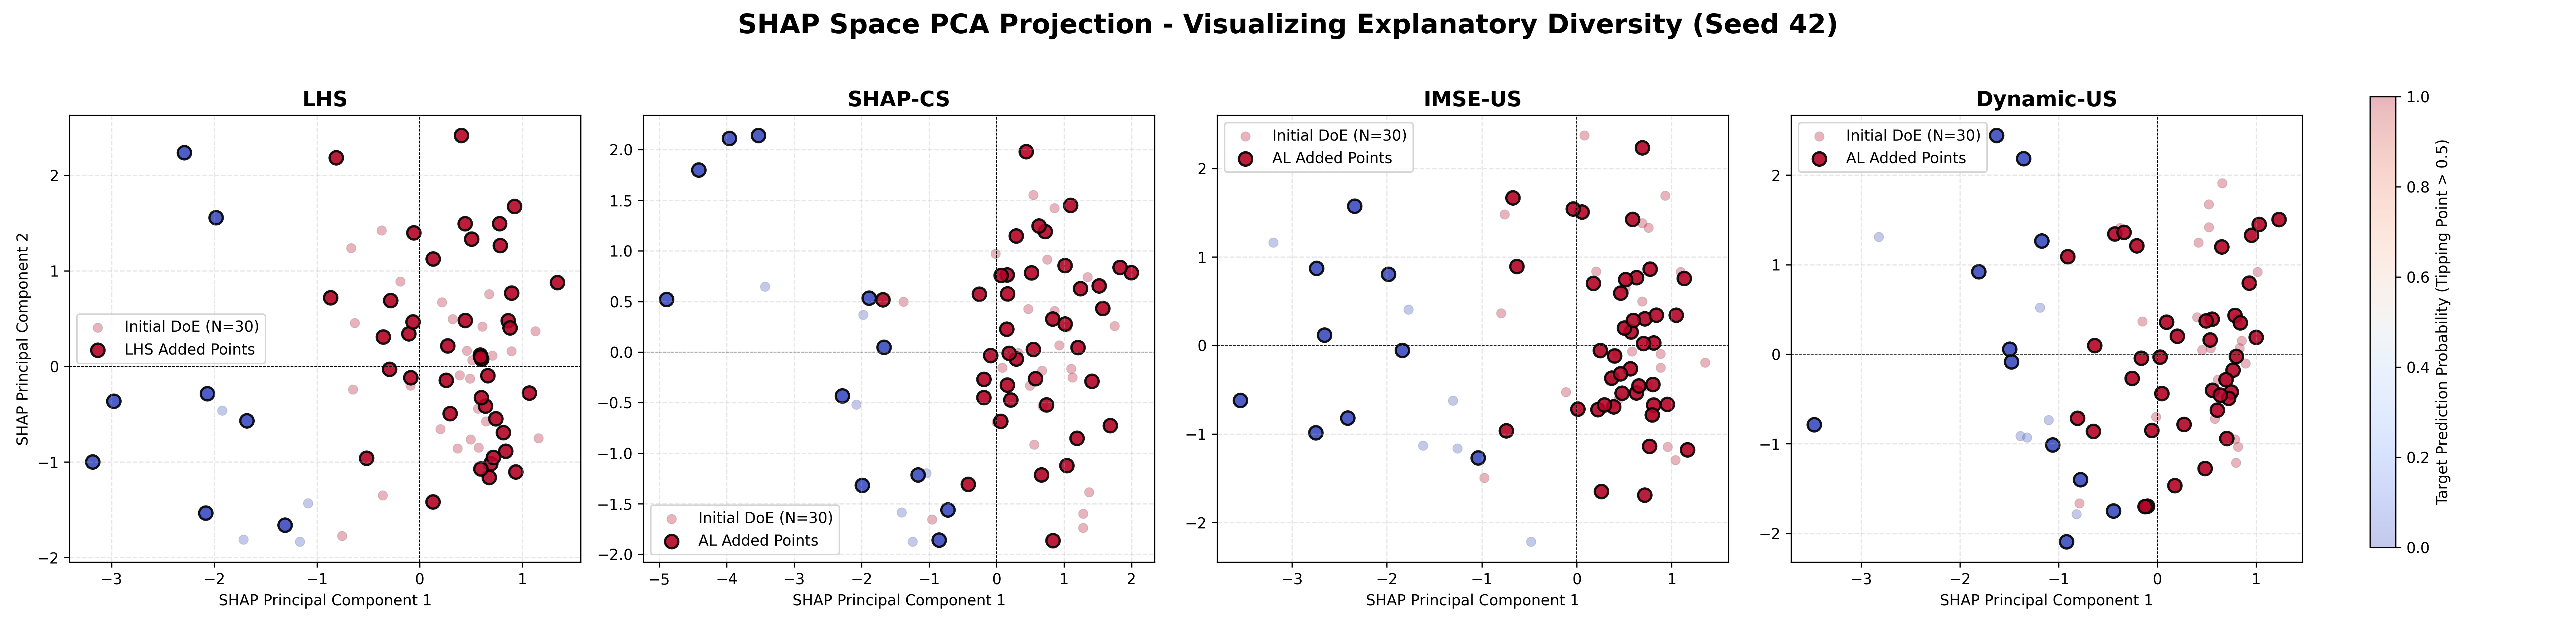
\includegraphics[width=\textwidth]{Images/MASTIO/tipping_points_pca_final_shap.png}
        \caption{MASTIO Final SHAP Space}
    \end{subfigure}
    \caption{By securing physical boundaries before pivoting to explanatory novelty, Dynamic-US identifies the true underlying transition boundaries better than pure SHAP novelty search, which often gets trapped in inaccurate surrogate spaces.}
    \label{fig:pca_final}
\end{figure}

\subsection{Impact on Output Space and Dual Efficiency}
The ability to map the explanatory boundaries translates directly into discovering extreme variations in the output space.
\begin{figure}[hbt!]
    \centering
    \begin{subfigure}{0.49\textwidth}
        
\includegraphics[width=\textwidth]{Images/Schelling/tipping_point_distribution.png}
        \caption{Schelling Output Space}
    \end{subfigure}
    \begin{subfigure}{0.49\textwidth}
        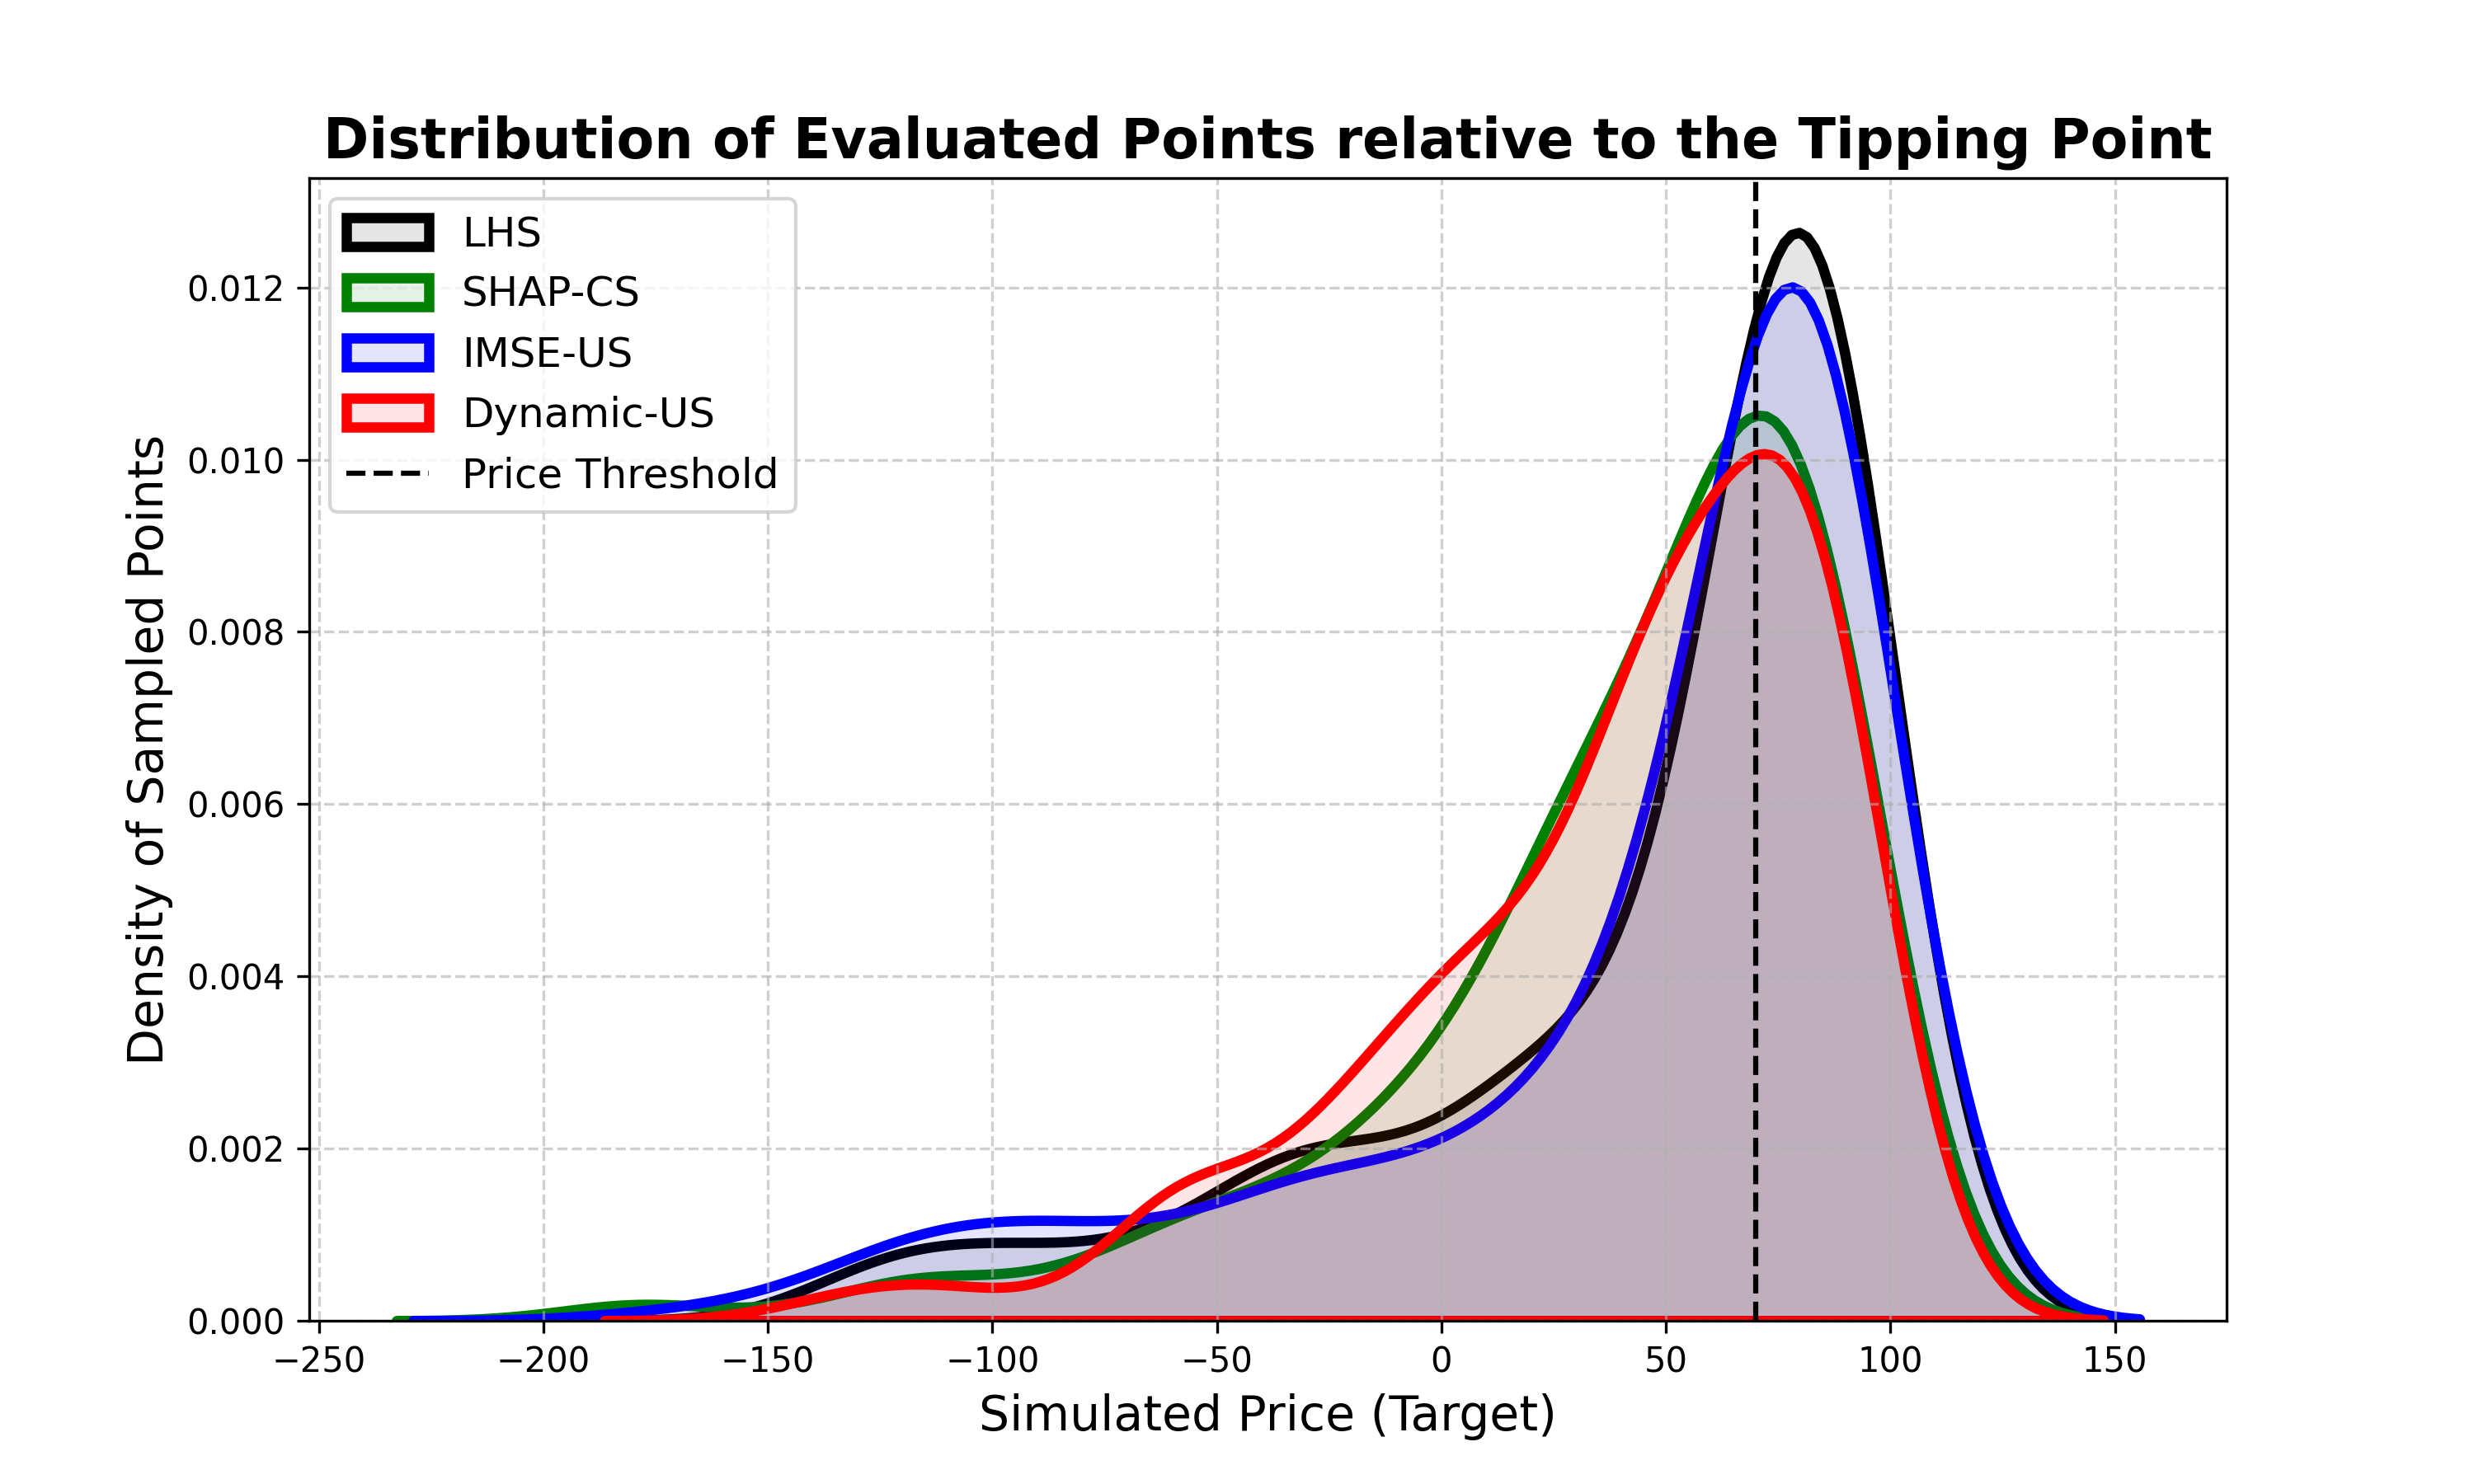
\includegraphics[width=\textwidth]{Images/MASTIO/tipping_point_distribution.png}
        \caption{MASTIO Output Space}
    \end{subfigure}
    \caption{Distribution of evaluated points relative to the physical tipping point threshold. The active learning loop explicitly populates the sparse, high-impact regions of the output.}
    \label{fig:output_space}
\end{figure}

Ultimately, evaluating the framework's convergence demonstrates its "dual space efficiency"—its capacity to rapidly acquire information in both the physical parameter space and the causal explanatory space. To rigorously quantify this without falling victim to the curse of dimensionality in continuous probability spaces, we measure the marginal Shannon entropy across all features. Each dimension is normalized between $[0, 1]$ and discretized into $N_{bins}=10$ intervals. The overall entropy $H$ is calculated as the average of the 1D marginal entropies: $H = - \frac{1}{M} \sum_{m=1}^M \sum_{k=1}^{N_{bins}} p_k \log p_k$. This formulation enables us to track the exploration dynamics robustly.
\begin{figure}[hbt!]
    \centering
    \begin{subfigure}{0.49\textwidth}
        
\includegraphics[width=\textwidth]{Images/Schelling/all_metrics_evolution.png}
        \caption{Schelling Metrics Evolution}
    \end{subfigure}
    \begin{subfigure}{0.49\textwidth}
        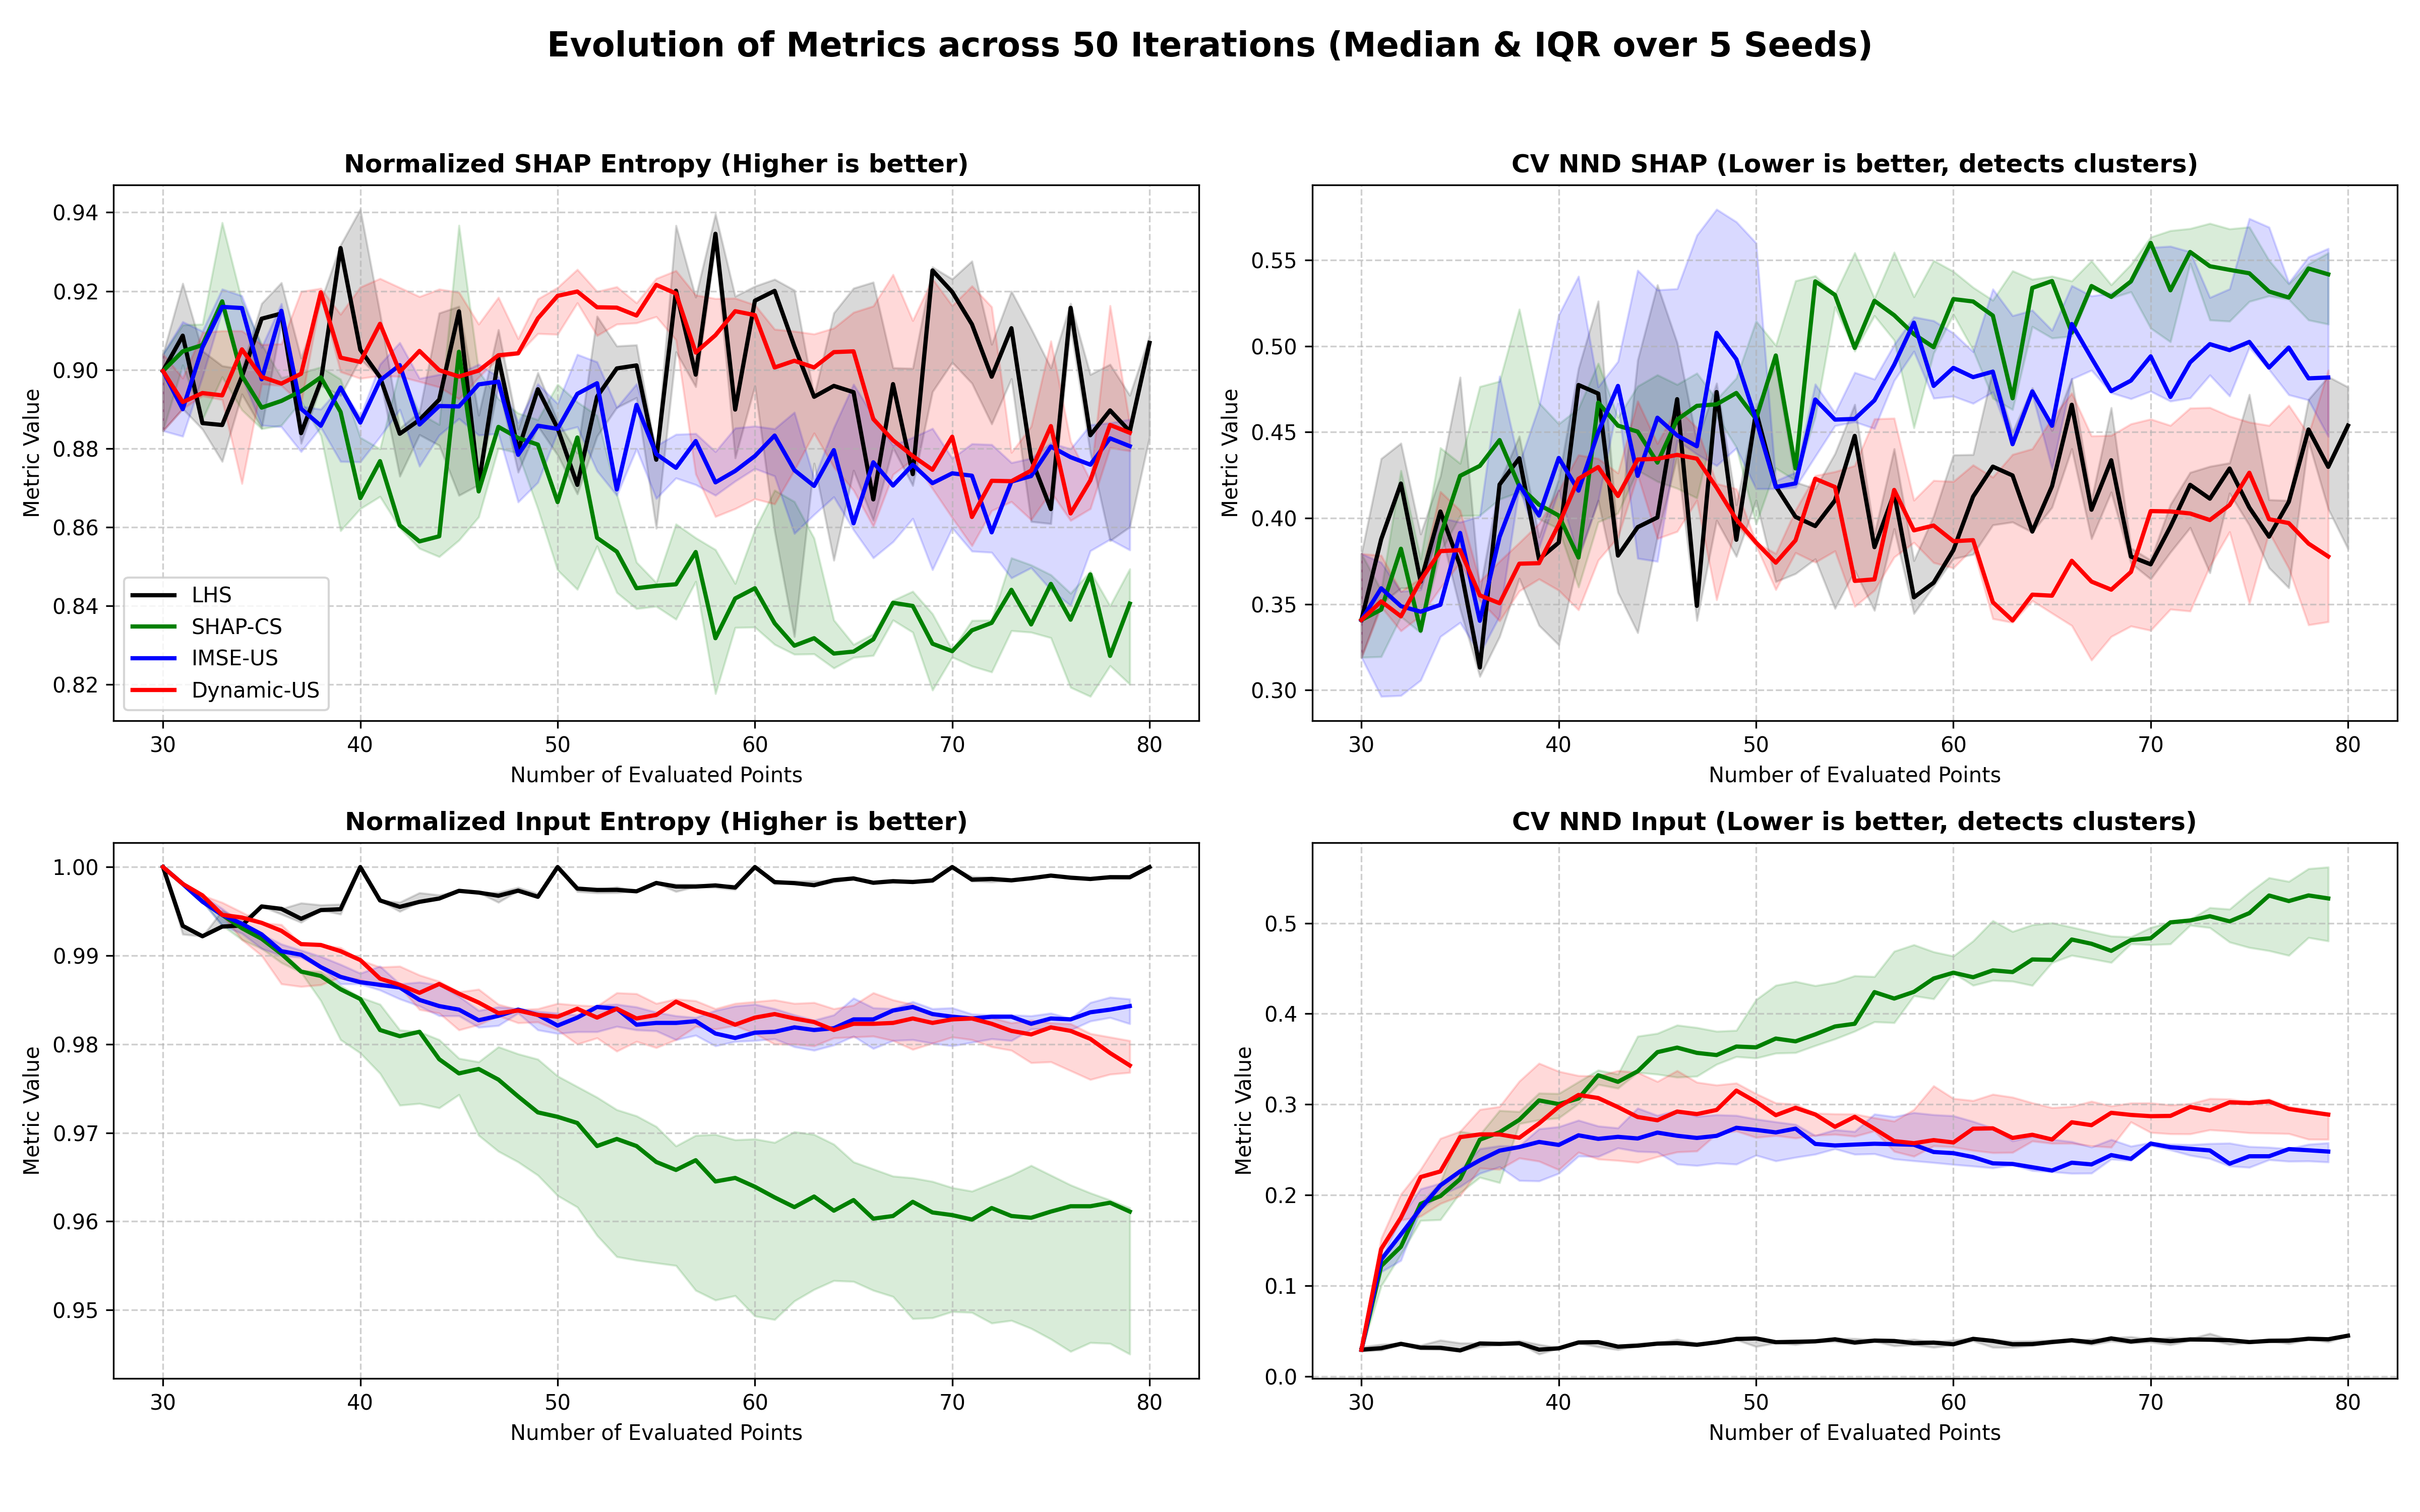
\includegraphics[width=\textwidth]{Images/MASTIO/all_metrics_evolution.png}
        \caption{MASTIO Metrics Evolution}
    \end{subfigure}
    \caption{Evolution of physical and explanatory entropy over iterations. Dynamic-US balances both objectives effectively.}
    \label{fig:metrics_evolution}
\end{figure}

\begin{figure}[hbt!]
    \centering
    \begin{subfigure}{0.49\textwidth}
        
\includegraphics[width=\textwidth]{Images/Schelling/dual_space_efficiency.png}
        \caption{Schelling Dual Efficiency}
    \end{subfigure}
    \begin{subfigure}{0.49\textwidth}
        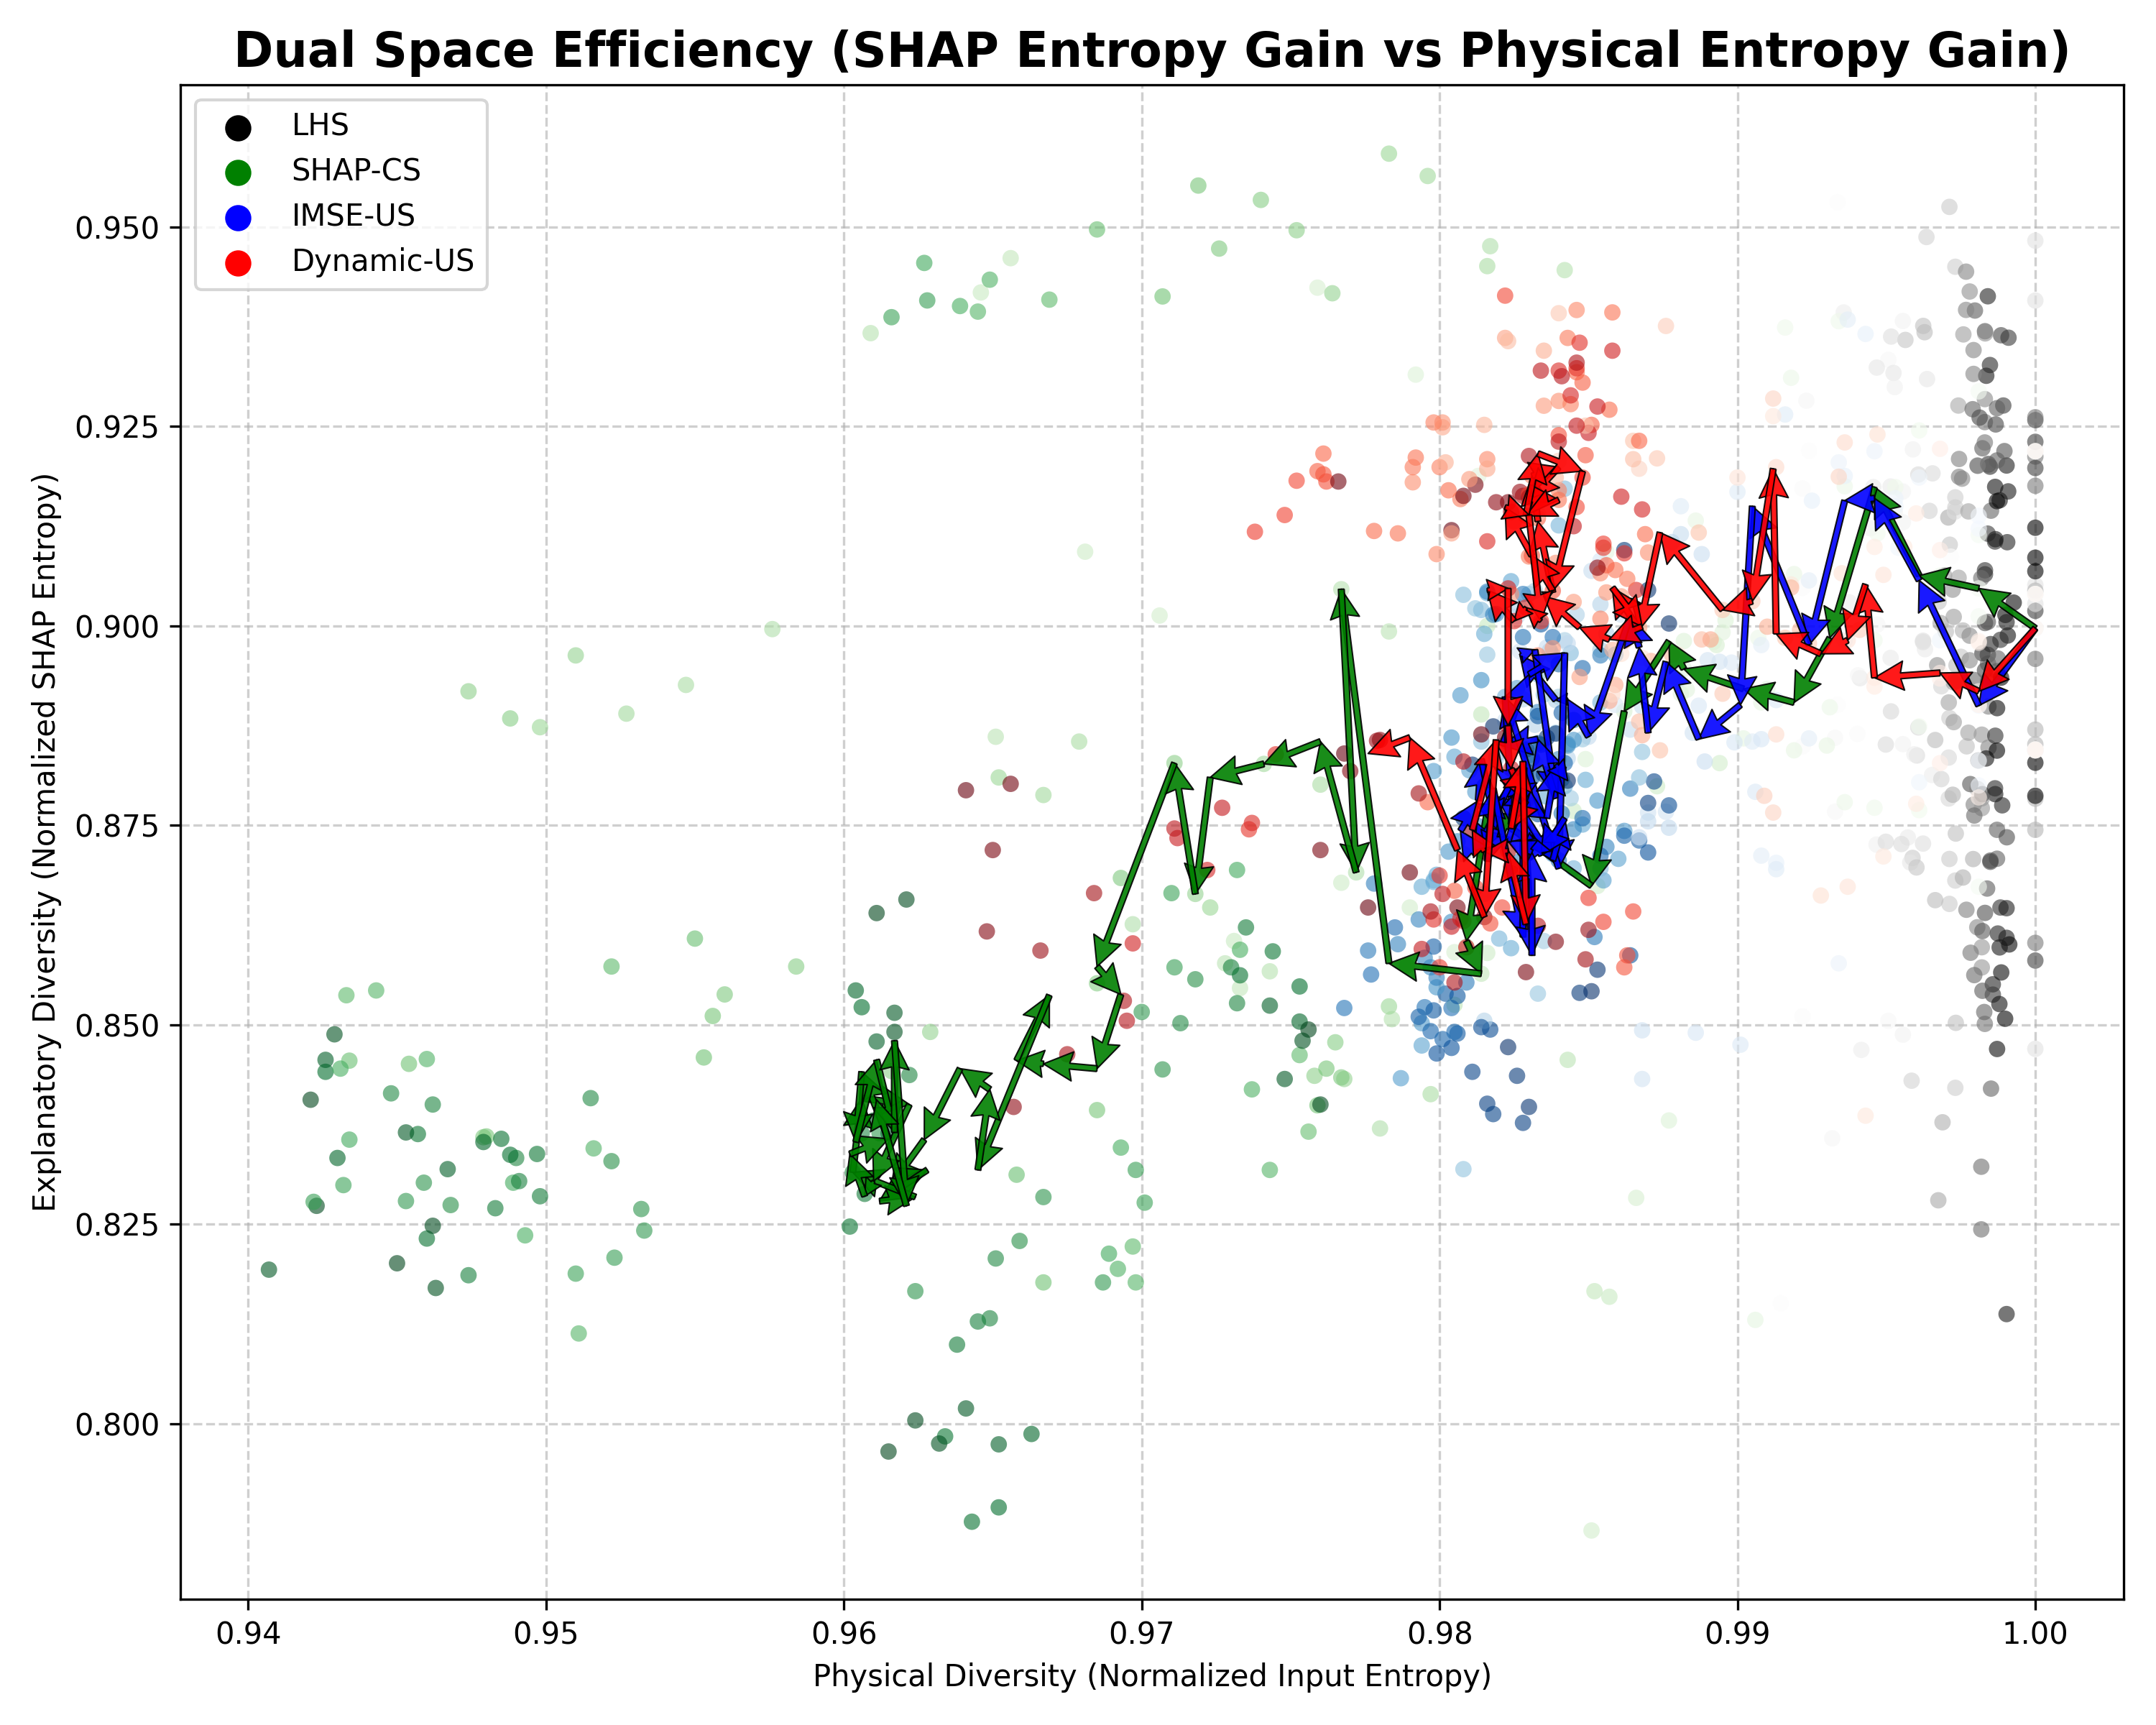
\includegraphics[width=\textwidth]{Images/MASTIO/dual_space_efficiency.png}
        \caption{MASTIO Dual Efficiency}
    \end{subfigure}
    \caption{SHAP Entropy Gain vs Physical Entropy Gain. Dynamic-US achieves a rapid, non-linear gain in explanatory entropy while preserving classical SUR space-filling properties.}
    \label{fig:dual_space}
\end{figure}

\section{Discussion and Scalability}
The primary advantage of this framework is its shift in focus from prediction accuracy to structural understanding[cite: 16]. By explicitly targeting "new explanations," modelers gain deeper engineering insights, improved model trustworthiness, and enhanced decision-support capabilities[cite: 16]. 

However, there are current scalability limitations. Computing ExactSHAP values, even on a fast GP surrogate, incurs a computational overhead of $\mathcal{O}(2^M)$ that scales exponentially with dimensionality $M$[cite: 50]. While the transition from classical KDE ($\mathcal{O}(N \cdot d)$ with complex bandwidth selection) to the Fast Cosine Proxy ($\mathcal{O}(N \log N)$) resolved the novelty estimation bottleneck, surrogate inference remains the primary limiting factor for scaling to $M > 15$ parameters.

From an operations research perspective, several mathematical enhancements have been integrated to improve the robustness of the acquisition process. The highly multimodal and non-stationary nature of the SHAP novelty landscape indicated that continuous gradient-based solvers like SLSQP were prone to local minima. By employing a global Derivative-Free Optimization (DFO) approach—specifically, Differential Evolution initialized directly from the Space-Filling LHS candidates—the surrogate calibration and convergence are significantly improved. Future work could explore replacing the linear scalarization of the bi-objective optimization with Expected Hypervolume Improvement (EHVI) or NSGA-II to properly identify non-convex regions of the Pareto front.

Immediate next steps and future perspectives for this research include:
\begin{itemize}
    \item \textbf{Exploiting Additive GP Kernels:} By leveraging the additive properties of specialized GP kernels (e.g., GP-SHAP), exact Shapley values could theoretically be computed analytically in $\mathcal{O}(M^2)$, bypassing the combinatorial explosion.
    \item \textbf{Neural Surrogate Models:} Transitioning from Gaussian Processes to Neural Surrogates (Multi-Layer Perceptrons). With neural surrogates, feature importance gradients can be extracted almost instantly via backpropagation ($\mathcal{O}(1)$ relative to inference), fully eliminating the SHAP bottleneck while maintaining a differentiable acquisition landscape.
    \item \textbf{Heteroscedastic Aleatoric Noise:} Transitioning from sequential mean stabilization to a fully Stochastic Kriging framework to natively integrate ABM variance into the acquisition function, as tipping points are often heralded by critical slowing down (variance explosion).
    \item Expanding the evaluation to include other diverse test cases to ensure generalization[cite: 116].
\end{itemize}

\section{Conclusions}
We have presented a black-box active learning framework that leverages surrogate modeling and Explainable AI to drive the exploration of complex systems[cite: 19]. By structuring an active learning loop around the maximization of explanatory diversity, the algorithm efficiently uncovers distinct causal mechanisms and rare behavioral regimes within high-dimensional parameter spaces.

Ultimately, this explainability-driven approach provides a pathway from raw simulation data to actionable, interpretable insights for complex decision-making processes[cite: 13, 16].

\section*{Conflict of interest}
The authors have no conflict of interest to declare.

\section*{Data availability and replication}
The codes and data used to produce the results are open-source and available online: {\url{https://github.com/ANR-MIMICO/SMPT_XAI}}.

\section*{Acknowledgements}
This work has been performed in the framework of the MIMICO research project funded by the Agence Nationale de la Recherche (ANR) n$^\text{o}$ ANR-24-CE23-0380. 

%\newpage
\bibliographystyle{plain}
\bibliography{sn-bibliography.bib}
%, biblio_ext.bib}
\pdfbookmark[1]{References}{sec-refs}

%\break
\appendix

\section{App.A}
\end{document}
